\section{Results}
\label{sec:800}

\Cref{fig:omp,fig:tbb} show the speedups measured for both the OpenMP and the TBB versions. As expected and explained in \cref{sec:400}, no speedups were expected, due to the extremely naive approach.

\begin{figure}[!htp]
	\centering
	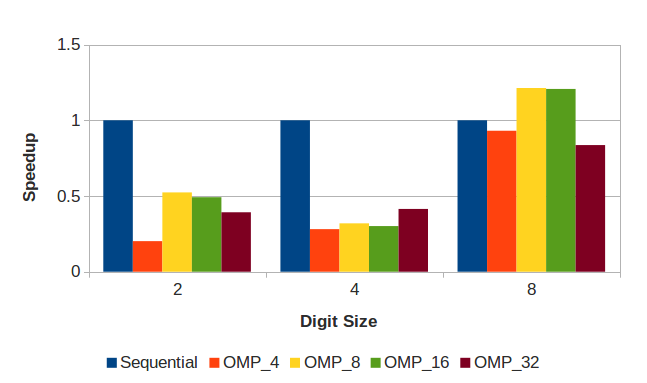
\includegraphics[width=\columnwidth]{plot-omp}
	\caption{Speedup results for OpenMP. Only the largest test case is shown}
	\label{fig:omp}
\end{figure}

OpenMP results show that speedups are only attained for 16 threads, with a digit size of 8 bits. However, a speedup of 1.2 with 16 threads is mostly insignificant, and it does not change the fact that the parallelization approach has problems.

\begin{figure}[!htp]
	\centering
	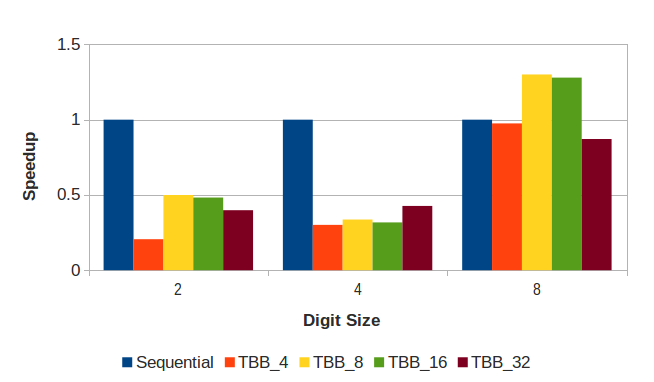
\includegraphics[width=\columnwidth]{plot-tbb}
	\caption{Speedup results for Threading Building Blocks. Only the largest test case is shown}
	\label{fig:tbb}
\end{figure}

Results for the equivalent tests on TBB show nearly the same values, with variatons not large enough to consider significant. This was expected since the parallelism approach did not change, only the underlying thread management library did, and if that would be a reason for significant performance differences, it would mean that the thread management of the slower one suffered from performance issues. This is not the case. Although particular overheads for library initialization and thread  spawning were not measured, total application time was measured, and did not show significant differences between OpenMP and TBB.

As for the results, it should also be noted that, even though no real performance gains can be achieved with the naive implementation, it can serve as a basis for a more robust approach, for example, using the suggested method of iterating by chuncks and synchronizing every thread between them. Also, results for 32 threads show an even worse performance decrease compared to other tests. This is due to the fact that 32 threads requires the node to try to take advantage of Hyper-Threading, which most of the cases ens up hurting performance, as can be seen by the results shown.

\subsection{OpenMP vs TBB}
\label{sec:810}

\Cref{fig:both-small,fig:both-big} show a comparison of the speedups achieved with both parallel implementations. Since the actual speedup is not demonstrative of the effectiveness of the libraries, because it is limited by the naive implementation, this serves to show that, from the two implementations, which are as much similar as it could be possible when using two different libraries, TBB seems to provide better results.

\begin{figure}[!htp]
	\centering
	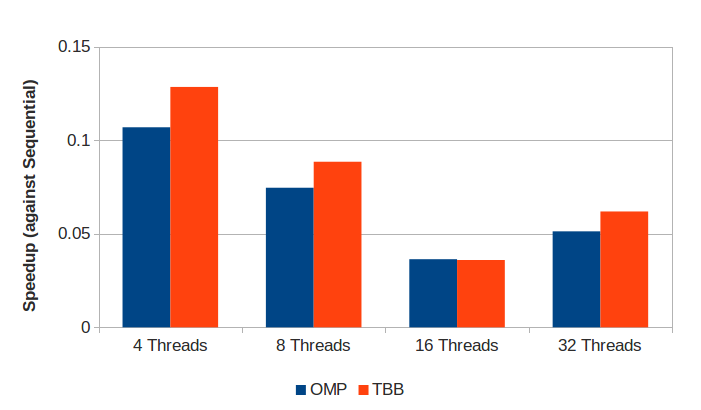
\includegraphics[width=\columnwidth]{plot-both-small}
	\caption{OpenMP vs TBB comparison on the smallest test case}
	\label{fig:both-small}
\end{figure}

\begin{figure}[!htp]
	\centering
	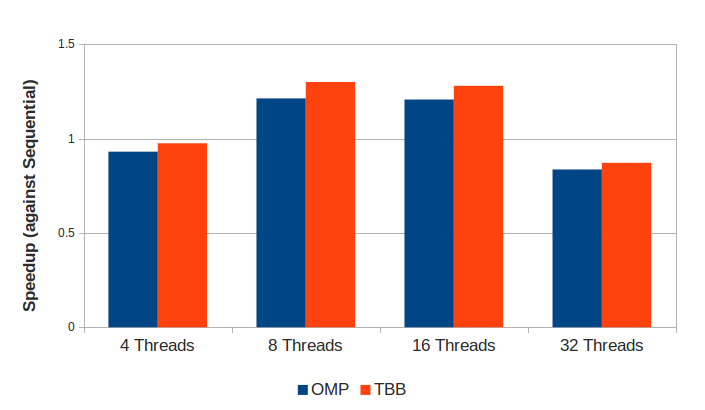
\includegraphics[width=\columnwidth]{plot-both-big}
	\caption{OpenMP vs TBB comparison on the largest test case}
	\label{fig:both-big}
\end{figure}

\Cref{fig:both-small} shows the speedup of each one for the smallest test case ($2^{11}$ keys) and \cref{fig:both-big} for the biggest test case ($2^{27}$ keys). In both cases, and also in the intermidiate ones that are not shown in this document, TBB managed to provide better speedups.

With a better parallel implementation, it could be possible that this small difference in speedup could escalate to a larger difference, but there was no way to prove that with the current implementation.